\section*{Quetions 4}

For question 4 we are tasked with created the best possible
kNN classifier given the data provided. To achieve that we took a different
approach with the Data and Model Selection.

{\bf For the data}, instead of using the train and test data provided as separate datasets,
we labeled and joined all data provided in a single dataset. The feature data was then scaled, so
both features have mean 0 and variance 1.

As for {\bf model selection} we then used a cross validation approach, where we tried different
kNN models with different k, hyperparameters and different metrics until we got the best
possible cross validation training error, and then trained the best model on all the data.

As reference, the best perfoming model of previous questions, the kNN with k=30 using
{\it Euclidean} metric has a cross validation error of $0.19 \pm 0.01$

One notable attempt was exponentially weighting the distances closes to the ``center'' of the feature space.
The center was determined by cross validation search to be around $center=(1.3, 1.5)$, and the feature vectors were
weighted by $exp(0.04*d(\bar{x}, center))$ where $d(\bar{x}, center)$ is the distance between the feature vector
$\bar{x}$ and the center. This is effectively a \textit{manifold based metric} that looks like a valley. The
points closer to the center are treated as if they were close together, and points far from the center
are ``uphill'', and further away. The final cross validation error for this approach was $0.165$, significantly
better than the \textit{Euclidean} or \textit{Manhattan} metrics


Additionally, we implemented the top ranked 5 metrics in the publication {\it Prasath, V. B. Surya, et al. “Distance and Similarity Measures Effect on the Performance of K-Nearest Neighbor Classifier -- A Review.” Big Data, vol. 7, no. 4, Dec. 2019, pp. 221–48.}. The ranking with noise set to 20\% was chosen
as reference for the 5 best performing metric. From those, the Hassanat Metric (defined by equation \ref{eq:HasD}, was also the top performing metric on our dataset
in our cross validations tests, with a cross validation error of $0.156 \pm 0.009$ for k=17.

\begin{equation}
HasD(\bar{x},\bar{y}) = \sum_{i=1}^2 D(x_i, y_i)
\label{eq:HasD}
\end{equation}

Where,

\begin{equation*}   
D(x_i,y_i) = 
     \begin{cases}
       min(x_i,y_i) \geq 0 & \quad 1 - \frac{1+min(x_i, y_i)}{1+min(x_i, y_i)} \\
       min(x_i, y_i) < 0 & \quade 1 - \frac{1+min(x_i, y_i)+|min(x_i, y_i)|}{1+max(x_i, y_i)+|min(x_i, y_i)|}
     \end{cases}
\end{equation*}

After the Hassanat Metric provided the best results, we trained it on all of the data,
including the ``test'' data provided, because of that we can't give an assessment of the model
beyond the cross validation trainig error. 

\renewcommand{\thefigure}{13}
\begin{figure}[h!]
    \centering
    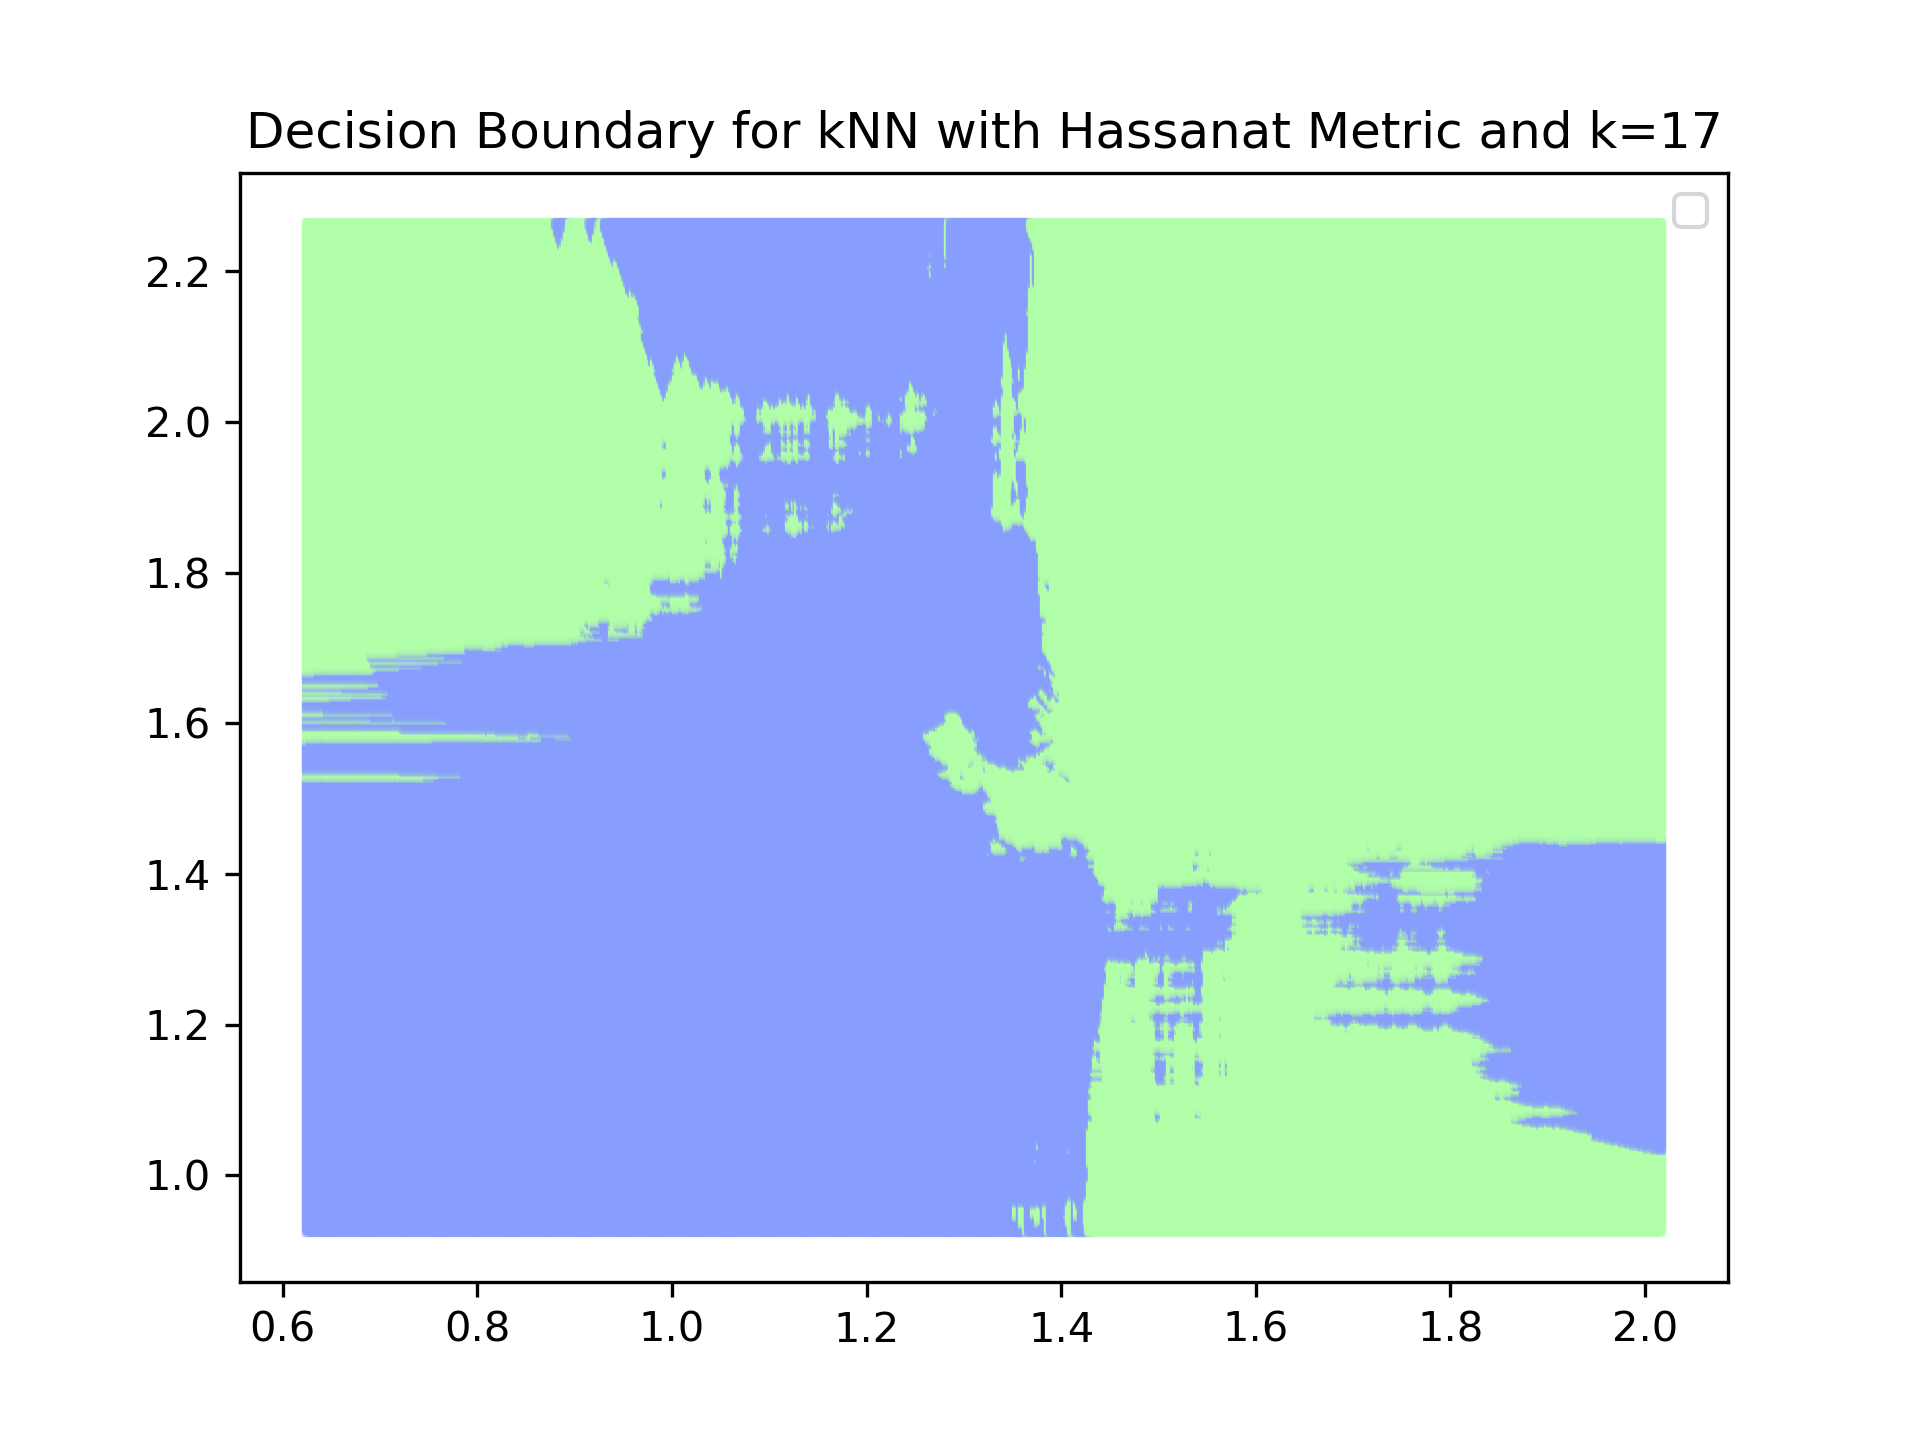
\includegraphics[width=\singleWidth]{Graphs/Q4.png}
    \caption{Classification region for kNN with Hassanat Metric for k=17, with sNC in green, and sDAT in blue}
    \label{fig:Q4}
\end{figure}





